\iflanguage{ngerman}
{\chapter{Konzeption}}
{\chapter{Concept}}
\label{sec:concept}

\section{Framework}
Die gesamte Implementation wird ein Plugin für das CGVF.
Dabei will Ich möglichst viele Schnittstellen auf dem Framework nutzen.
Eine der wichtigsten Schnittstellen ist das eingebaute GUI-System, das für die Demo-Anwendung zum Einsatz kommen wird.

\section{SDFs}
Große Teile der Arbeit werden sich auf SDFs stützen, da diese der beste Weg sind um Vektor-Graphiken auf Fragmentbasis darzustellen.
Außerdem gibt es Möglichkeiten komplexere Graphiken mit Rasterisierung in Teil Graphiken zu unterteilen, wie in \cite{Nehab2008} beschrieben.


\section{Referenzsystem}
Alle Elemente des Plots, die auf der zugrunde liegenden Geometrie dargestellt werden brauchen zur Bestimmung ihrer Position ein Referenzsystem.
Dieses Referenzsystem ist im Texturraum der Geometrie.
Also können wir z.B. die UV-Koordinaten nutzen, die uns GLSL bereitstellt.
Der UV-Koordinatenraum erstreckt sich von (0.0, 0.0) zu (1.0, 1.0).
Ich bevorzuge jedoch ein Referenzsystem, das sich von (-1.0, -1.0) bis (1.0, 1.0) erstreckt und bei dem der Punkt (0.0, 0.0) genau in der Mitte liegt.
Das ist auch das Referenzsystem von dem Ich in der restlichen Arbeit ausgehen werde.

\section{Graphen}
Es soll die Möglichkeit geben, statt nur einzelner Punkte, auch Kontinuierliche Graphenlinien zu Zeichnen.
Punkte und Linien sollten auch kombiniert eingesetzt werden können.
Abbildung \ref{fig:dots} veranschaulicht diese Darstellungsmöglichkeiten.
Der einfachste Weg so eine Linie darzustellen ist, das einfache erzeugen eines Liniensegments zwischen zwei, nebeneinander liegenden Punkten im Datensatz für den Graphen.
Ein Beispiel für so eine Darstellung sieht man in Abbildung \ref{fig:graphs}.
\begin{figure}[ht]
	\centering
	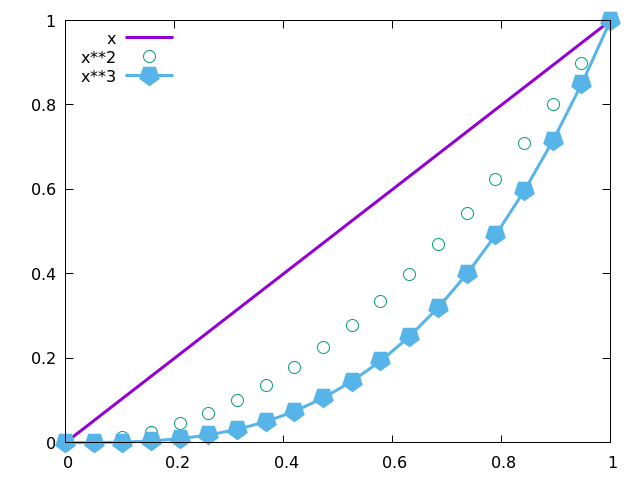
\includegraphics[width=0.6\textwidth]{fig/dots.png}
	\caption{Gnuplot 5 \cite{Phillips2020} p.47}
	\label{fig:dots}
\end{figure}
\FloatBarrier
\begin{figure}[ht]
	\centering
	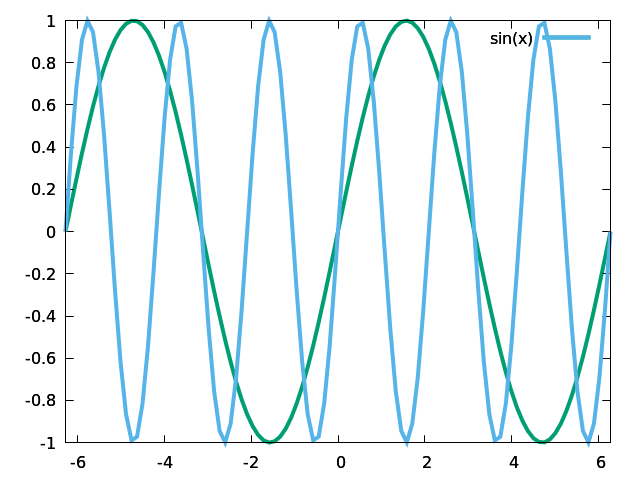
\includegraphics[width=0.6\textwidth]{fig/segments.png}
	\caption{Gnuplot 5 \cite{Phillips2020} p.41}
	\label{fig:graphs}
\end{figure}
\FloatBarrier

\section{Dekoration}
\subsection{Grid}
Der Plot soll noch weitere Bestandteile haben außer den Graphen.
Eine wichtige Dekoration ist ein Grid auf dem gesamten Plot zur Orientierung, wie in Abbildung \ref{fig:grid}.
\begin{figure}[ht]
	\centering
	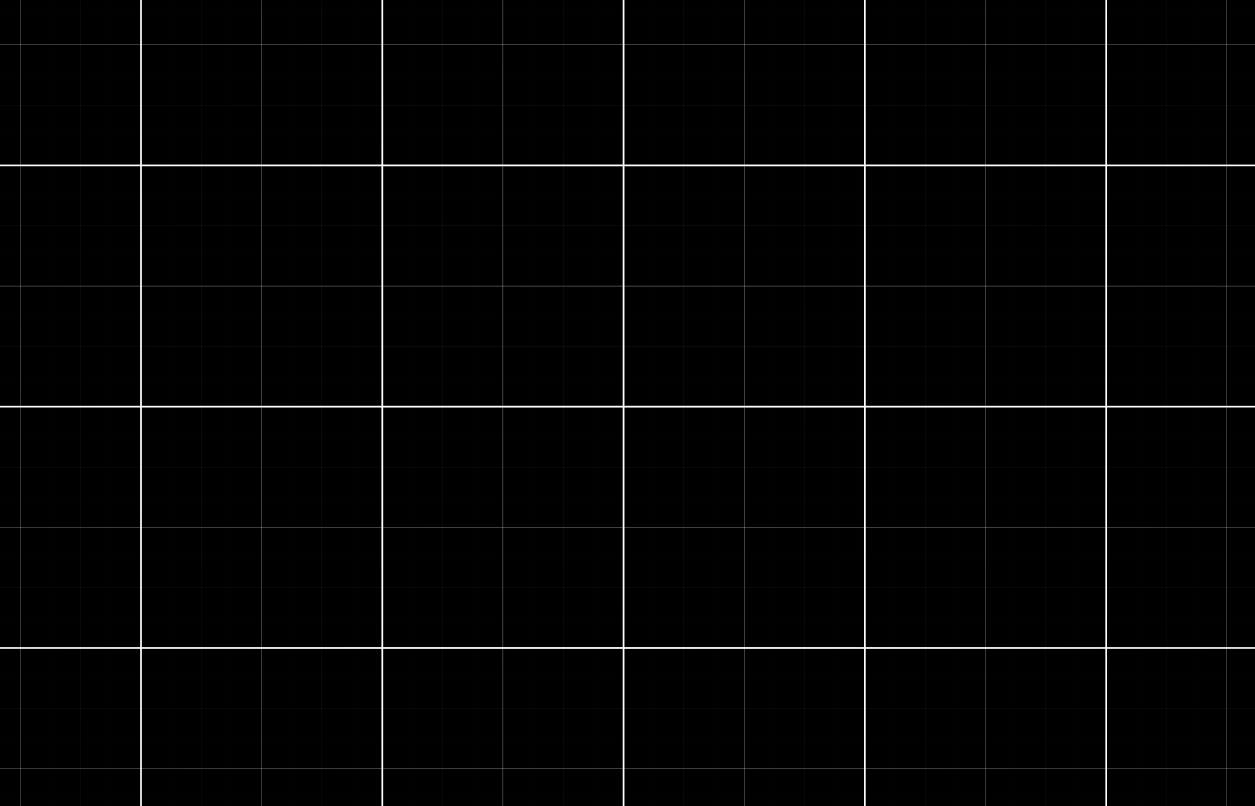
\includegraphics[width=0.6\textwidth]{fig/grid.png}
	\caption{Gnuplot 5 \cite{Phillips2020} p.31}
	\label{fig:grid}
\end{figure}
\FloatBarrier
Natürlich gibt es neben einem statischen Raster auch andere Möglichkeiten für ein Grid.
Für ein dynamisches Grid, das seine Auflösung an die Zoomstufe anpassen kann braucht man einen Referenzpunkt.
Ich werde versuchen ein Grid zu Implementieren, das sich and der Position im 3D-Raum orientiert.
Dabei sollen mehr Grid-Linien erscheinen, desto näher man heran geht.
Die Auflösung des Rasters sollte großer werden wenn weiter weg geht und feinen Rasterlinien sollten verschwinden.
\subsection{Tickmarks}
An beiden Hauptachsen sollte es Tickmarks geben die eine alternative Orientierungsmöglichkeit zum Grid bieten.
Diese Tickmarks könnten, genau wie das Grid ebenfalls dynamisch sein und sich an die Zoomstufe anpassen.
Dabei würde die Unterteilung zwischen den Tickmarks beim heranzoomen immer kleiner.
\subsection{Färbung}
Alle Dekorationen sollten die Möglichkeit haben, sie beliebig einzufärben, um verschiedene Aspekte visuell hervorheben zu können.
\subsection{Beschriftung}
Beschriftungstext an Achsen, Graphen oder sogar einzelnen Tickmarks ist wichtig für das herauslesen von Größen und anderen Informationen von Plots.
Der Text könnte dabei auch 'prozedural' im Fragment-Shader erzeugt werden.
Dazu müssen Glyphen aus einem SDF-Atlas geladen werden.
Die Erstellung eines solchen Atlas ist z.B. mit der Implementierung 'msdfgen' \cite{msdfgen2021} möglich.
Um bessere Ecken und Kanten bei niedrig aufgelösten SDF-Texturen zu haben, bieten sich Multi-Channel-SDFs an, wie in diesem Paper beschrieben \cite{Green2007}.

\section{Raumtransformation}
Eine weitere nützliche Funktion, wäre eine Auswahl aus verschiedenen Achsenräumen.
So könnte man neben dem normale Raum auch logarithmisch oder exponentiell wachsende Achsen haben.

\section{Interaktion}
Die Implementierte Demo soll dem Nutzer die Möglichkeit geben beliebig viele Graphen im selben Plot darzustellen und diese auch individuell anpassen zu können.
Der Nutzer muss auch in der Lagen sein im 3D-Raum mit dem Plot zu interagieren durch einen adaptive Grid-Auflösung, die sich an der Distanz zur Kamera orientiert.
